\documentclass[openany,a4paper,oneside,11pt]{article}

\usepackage{amsmath,amsfonts,amsthm,physics,braket,indentfirst}
\usepackage{float}

\usepackage[a4paper,
            left=3cm,
            right=3cm,
            top=3cm,
            bottom=3cm]{geometry}

\usepackage{lipsum}

\usepackage{graphicx}

\usepackage{hyperref}
\hypersetup{
	colorlinks=true,       	
	linkcolor=blue,          	
	citecolor=blue,        		
	urlcolor=blue}
\usepackage{url}

\newtheorem{alg}{Algorithm}
\newtheorem{exe}{Exercise}

\title{Numerical propagation in turbulent media}
\author{M. Gil de Oliveira}
\date{\today}

\begin{document}

\maketitle


\section{Propagation in free space}

Although we aim to study the propagation of light in turbulent media, it is important to first understand how light propagates in free space. This will provide us with a solid foundation for understanding the effects of turbulence on light propagation.

\subsection{The paraxial wave equation}

Our starting point will be the wave equation for the electric field, which is derived from Maxwell's equations. In free space, the wave equation can be expressed as
\begin{equation}
    \label{eq:wave equation}
    \nabla^2 E - \frac{1}{c^2} \partial_t^2 E = 0,
\end{equation}
where $E$ is the electric field, which we assumed to have a fixed polarization, $c$ is the speed of light in vacuum, and $\nabla^2$ is the Laplacian operator in three-dimensional space. 

A well known class of solutions are the plane waves $E(\mathbf{r}, t) = E_0 e^{i(\mathbf{k} \cdot \mathbf{r} - \omega t)}$ satisfies this equation, where $\mathbf{k}$ is the wave vector, $\omega$ is the frequency, and $E_0$ is a constant amplitude. The norm of the wave vector is related to the frequency $\omega$ by $ck = \omega$. These solutions have a well-defined direction of propagation defined by the wave vector $\mathbf{k}$, which we assume to be the $z$ direction, i.e., $\mathbf{k} = k \hat{\mathbf{z}}$.

Nonetheless, this class of solutions is nonphysical, as the electric field is not localized in space and contains an infinite amount of energy. A more physically relevant solution can be obtained by considering a field of the form
\begin{equation}
    E(\mathbf{r}, t) = u(\mathbf{r}) e^{i(kz - \omega t)},
\end{equation}
where $u(\mathbf{r})$ is a complex function describing an envelope that modulates the plane wave. By substituting this expression into the wave equation \eqref{eq:wave equation}, we obtain
\begin{equation}
    \nabla^2 u + 2ik \partial_z u= 0.
\end{equation}

\begin{figure}[]
    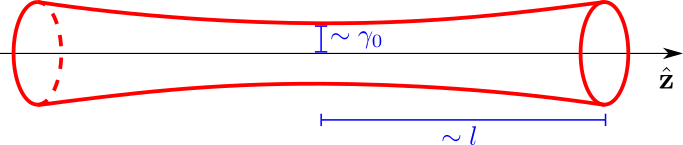
\includegraphics[scale=0.7]{feixe_paraxial.png}
    \centering
    \caption{Envelope of a paraxial beam.}
    \label{fig: paraxial beam}
\end{figure}

The typical envelope of a laser beam is shown in Fig. \ref{fig: paraxial beam}. The envelope $u(\mathbf{r})$ varies slowly along the $z$ direction. More precisely, the variation of $u$ in the $z$ is much smaller than the scale of variation defined by the wavenumber $k$. Therefore, we will assume that $\partial_z^2 u \ll k \partial_z u$, which allows us to neglect the second derivative with respect to $z$ in the wave equation. This leads us to the paraxial wave equation
\begin{equation}
\label{eq:paraxial}
    \nabla^2_T u + 2ik \partial_z u = 0,
\end{equation}
where $\nabla^2_T$ is the Laplacian operator restricted to the transverse plane, i.e., $\nabla^2_T = \partial_x^2 + \partial_y^2$.

\subsection{Solution of the paraxial wave equation}

The paraxial wave equation \eqref{eq:paraxial} is a partial differential equation that describes the propagation of light beams in the paraxial approximation. We want to find a solution for this equation, which will allow us to understand how light propagates in free space. In particular, we want to find a solution for the electric field envelope $u(x,y,z)$ given an initial condition $u(x,y,0)$ at $z=0$.

As it the equation is, the most straightforward way to solve it is to use the Fourier transform. Let us then define the Fourier transform of $u(x,y,z)$ as
\begin{equation}
\label{eq:fourier_transform}
    \tilde{u}(k_x, k_y,z) = \int_{\mathbb{R}^2} dx dy \ e^{-i(k_x x + k_y y)} u(x,y,z),
\end{equation}
which can be inverted as
\begin{equation}
\label{eq:inverse_fourier_transform}
    u(x,y,z) = \frac{1}{(2\pi)^2} \int_{\mathbb{R}^2} dk_x dk_y \ e^{i(k_x x + k_y y)} \tilde{u}(k_x, k_y,z).
\end{equation}
Substituting this expression into the paraxial wave equation \eqref{eq:paraxial}, we obtain
\begin{equation}
    \left( -k_x^2 - k_y^2 + 2ik \partial_z \right) \tilde{u}(k_x, k_y,z) = 0.
\end{equation}
This is a simple ordinary differential equation in $z$ for each fixed pair $(k_x, k_y)$. The solution can be written as
\begin{equation}
\label{eq:solution_paraxial_fourier}
    \tilde{u}(k_x, k_y,z) = \tilde{u}(k_x, k_y,0) e^{-i(k_x^2 + k_y^2)z/2k}.
\end{equation}

This provides a step-by-step algorithm for solving the paraxial wave equation:
\begin{alg}[Angular spectrum method]
\leavevmode
\begin{enumerate}
    \item Compute the Fourier transform $\tilde{u}(k_x, k_y,0)$ of the initial condition $u(x,y,0)$ using \eqref{eq:fourier_transform}.
    \item For each pair $(k_x, k_y)$, compute the solution $\tilde{u}(k_x, k_y,z)$ using the formula \eqref{eq:solution_paraxial_fourier}.
    \item Finally, compute the inverse Fourier transform to obtain the solution $u(x,y,z)$.
\end{enumerate}
\end{alg}

This is the angular spectrum method, which is a powerful technique for solving the paraxial wave equation. It allows us to compute the solution in the Fourier domain, where the equation becomes much simpler to solve. This is the basis for the method we will use to numerically simulate the propagation of light in turbulent media.

An equivalent way to express the solution of the paraxial equation, that is more simple from the analytical point of view, is obtained by substituting the expression \eqref{eq:solution_paraxial_fourier} into the inverse Fourier transform \eqref{eq:inverse_fourier_transform} and applying the convolution theorem. \footnote{This theorem states that the Fourier transform of convolution is the product of the Fourier transforms.} This leads to the following expression for the solution:
\begin{equation}
\label{eq:fresnel_diffraction}
    u(x,y,z) = \frac{k}{2\pi i z} \int_{\mathbb{R}^2} dx^\prime dy^\prime u(x^\prime,y^\prime,0) e^{ik\left[ (x-x^\prime)^2 + (y-y^\prime)^2 \right] / 2z}.
\end{equation}

This is the so-called Fresnel diffraction integral \cite{goodman2017introduction, schmidt2010numerical}.

\begin{exe}
    Apply the Fresnel diffraction integral to solve the paraxial wave equation for the initial condition
    \begin{equation}
        u(x,y,0) = e^{-(x^2+y^2)/w^2},
    \end{equation}
    where $w$ is a constant that defines the width of the beam (waist). 
\end{exe}

The Fresnel diffraction formula can be simplified when the distance $z$ is sufficiently large. In fact, assume that our initial condition $u(x,y,0)$ is mostly localized in a disk of radius $w$ around the origin, i.e., $u(x,y,0) \approx 0$ for $x^2+y^2 > w^2$. Then, when $z \gg kw^2/2$, the term $k[(x^\prime)^2 + (y^\prime)^2] / 2z$ in the exponent of \eqref{eq:fresnel_diffraction} does not contribute to the integral, and we can approximate the Fresnel diffraction integral as
\begin{equation}
    u(x,y,z) \approx \frac{k e^{ik\left( x^2 + y^2 \right) / 2z}}{2\pi i z} \int_{\mathbb{R}^2} dx^\prime dy^\prime u(x^\prime,y^\prime,0) e^{ik\left( xx^\prime + yy^\prime \right) / z}.
\end{equation}
This is known as the Fraunhofer diffraction integral, and it describes the far-field propagation of light. We can then see that, within the Fraunhofer approximation, the propagation of light can be understood as a Fourier transform of the initial condition $u(x,y,0)$, modulated by a quadratic phase factor that depends on the distance $z$.

\subsection{Analogy with quantum mechanics}

The paraxial wave equation \eqref{eq:paraxial} is analogous to the Schrödinger equation in quantum mechanics
\begin{equation}
    i \partial_t \psi(x, y, t) = -\frac{\hbar^2}{2m} \nabla^2 \psi(x, y, t),
\end{equation}
which describes the evolution of a free particle with wave function $\psi(x, y, t)$ in a two-dimensional space. The analogy is particularly useful because it allows us to use the same mathematical techniques to solve both equations. In fact, the angular spectrum method can be seen as a Fourier transform method for solving the Schrödinger equation, where the wave function $\psi$ plays the role of the electric field envelope $u$.

If we assume that our wave propagates through a medium with a space-dependent refractive index $n(x,y)$, the paraxial wave equation becomes may be approximated as
\begin{equation}
    \nabla^2_T u + 2ik \partial_z u + k^2(n^2 - 1) u = 0,
\end{equation}
which is analogous to the Schrödinger equation with a potential, i.e.,
\begin{equation}
    i \partial_t \psi(x, y, t) = \left( -\frac{\hbar^2}{2m} \nabla^2 + V(x,y) \right) \psi(x, y, t).
\end{equation}
This is what happens, for example, inside a waveguide, with the refractive index $n(x,y)$ being responsible for confining the light to a specific region of space, just like a potential well confines a quantum particle.

This analogy can also be extended to understand the imaging properties of lenses \cite{stoler1981operator}.

\subsection{Numerical solution}

From the analytical point of view, the Fresnel diffraction integral \eqref{eq:fresnel_diffraction} would be the most straightforward way to compute the solution of the paraxial wave equation. However, it is often not practical to compute this integral directly. Instead, we will use a numerical method based on the angular spectrum method, which is often more efficient from a computational point of view.

To simplify the notation, we will assume a single transverse dimension, i.e., we will consider the paraxial wave equation in 1 transverse dimension, with a solution $u(x,z)$. The extension to two transverse  is straightforward.

\subsubsection{Representing the solution numerically}

Although one is used to thinking of the solution $u(x,z)$ as a continuous function, in a computer we will have to represent it as a \textit{discrete} and \textit{finite} set of values. Usually, we represent the initial condition $u(x,0)$ as an array of values $u_m(0) = u(x_m, 0)$, where $m = 0, \ldots, N-1$, and $N$ is the total number of points in the array. The values of $x$ are then given by $x_m = m \Delta x$, where $\Delta x$ is the spacing between the points. Any numerical method will then compute (an approximation of) the solution at a later time $z$ as an array of values $u_m(z) = u(x_m, z)$. Then, we can only have access to samples of the solution that lie inside the interval $[0, L]$, where $L = N \Delta x$.

\subsubsection{Boundary conditions}

We can interpret the restriction to a finite interval $[0, L]$ in two different ways: we either assume that this is just a finite portion of the solution, which exists in the entire real line, or we assume that we are only seeking to solve the paraxial wave equation in the interval $[0, L]$. The first interpretation makes more physical sense for free space propagation, while the second one is more practical for numerical simulations, as we will see. An important difference is that, that, in the second case, we will have to impose boundary conditions at the edges of the interval, as the paraxial wave equation in itself is no longer sufficient to determine the solution uniquely. This is true for any partial differential equation defined in a finite domain. 

For example, a wave equation with one spatial dimension may model the propagation of a wave in a string. There are many possible behaviors for a wave pulse when it reaches the end of the string, and each of these behaviors corresponds to a different boundary condition. For example, if the string is fixed at the ends, we impose $u(0,t) = u(L,t) = 0$, which are the so-called Dirichlet boundary conditions. If the string is free at the ends, and we still want to have energy conservation, we impose the Neumann boundary conditions $\partial_x u(0,t) = \partial_x u(L,t) = 0$. These boundary conditions produce different solutions for the wave equation, whose differences are clearly seen in the reflection of a pulse on the edges: for Dirichlet boundary conditions, the reflected wave has a phase shift of $\pi$ (it gains a minus sign), while, for Neumann boundary conditions, there is no phase shift.

For propagation in free space, the physical solution exists everywhere, and there is no boundary on which to set conditions. Even so, as already said, it is more efficient to find a solution only on the finite domain $[0,L]$, and to assume \textit{periodic} boundary conditions $u(0,z) = u(L,z)$. For our case, this is indeed nonphysical, but, at is turns out, is a good approximation to the physical situation \textit{as far as all the intensity is concentrated far away from the edges of the interval}. We will then always have to keep an eye to this, and increase $L$ if necessary. This is a fair price to pay in order to be able to find an approximate solution efficiently.

\subsubsection{First attempt: the Fourier series}

As we are working on finite domain $[0,L]$, the Fourier transform \eqref{eq:fourier_transform} is simply not defined. Instead, as we assumed periodic boundary conditions, there is the close concept of a Fourier series
\begin{equation}
    \label{eq:fourier series}
    u(x,z) = \sum_{n=-\infty}^{\infty} \tilde{u}_n(z) e^{i k_n x}, \ \ \ k_n = \frac{2\pi n}{L},
\end{equation}
where the Fourier coefficients $\tilde{u}_n(z)$ are given by
\begin{equation}
    \tilde{u}_n(z) = \frac{1}{L} \int_0^L dx \ e^{-i k_n x} u(x,z).
\end{equation}

This is the equivalent of the Fourier transform for periodic functions, and it is defined in terms of a discrete sum over the wave numbers $k_n$, instead of continuous integral over wavenumbers. The Fourier coefficients $\tilde{u}_n(z)$ are complex numbers that encode the amplitude and phase of each harmonic component of the solution $u(x,z)$.

We may then proceed just as the continuous case, and substitute the Fourier series \eqref{eq:fourier series} into the paraxial wave equation \eqref{eq:paraxial}. This leads to a simple ordinary differential equation for each Fourier coefficient $\tilde{u}_n(z)$:
\begin{equation}
    \left( -k_n^2 + 2ik \partial_z \right) \tilde{u}_n(z) = 0.
\end{equation}
The solution of this equation is given by
\begin{equation}
    \tilde{u}_n(z) = \tilde{u}_n(0) e^{-i k_n^2 z / 2k},
\end{equation}
where $\tilde{u}_n(0)$ are the Fourier coefficients of the initial condition $u(x,0)$, which can be computed as
\begin{equation}
    \tilde{u}_n(0) = \frac{1}{L} \int_0^L dx \ e^{-i k_n x} u(x,0).
\end{equation}

All of these expressions actually provide exact solutions of the paraxial wave equation with periodic boundary conditions, and are analogous to the angular spectrum method. 

Nonetheless, there are still problems that do not allow us to use this method numerically. Note that the hypothesis of a finite domain turned the wave numbers from continuous to discrete, which is definitely a gain. Nonetheless, there are still an infinite amount of them, which, of course, cannot be handled by a computer.

Another problem of this approach is the following: as mentioned, we only have access to the initial condition $u(x,0)$ in a finite set of points, which may be arranged in a vector $u_m(0) = u(x_m,0)$. In order to compute the Fourier coefficients $\tilde{u}_n(0)$, we could try to approximate it as a Riemann sum
\begin{equation}
    \tilde{u}_n(0) \approx \frac{1}{L} \sum_{m=0}^{N-1} e^{-i k_n x_m} u_m(0) \Delta x = \frac{1}{N} \sum_{m=0}^{N-1} e^{-i 2\pi mn/N} u_m(0).
\end{equation}
Note that, in this approximation, the Fourier components will form a periodic sequence: $\tilde{u}_n(0) = \tilde{u}_{n+N}(0)$. Then, the series \eqref{eq:fourier series} cannot converge, as the coefficients of the series do not decay to zero. This periodicity makes sense from an "informational point of view", as we give $N$ points of information, and we can only expect to recover $N$ Fourier coefficients.

Although this approach does not work with finite data, it is an important step in the right direction. The approach we present in the next section is motivated by this discussion.

\subsubsection{Second attempt: the discrete Fourier transform}

The discussion will be based on the notes \cite{fftderiv}, which provides a detailed explanation of how to calculate derivatives based on the (Discrete) Fourier Transform. 

As we mentioned, in order to apply the angular spectrum method numerically, the spatial domain must be finite. This means that we will only be able to access the solution $u(x, z)$ inside a finite interval in $x$, say $x \in [0, L]$, where $L$ is the length of the interval. 
First, we need to recognize that any numerical implementation must handle discrete and finite data. The most straightforward way to proceed would then to implement the integrals in \eqref{eq:fourier_transform} and \eqref{eq:inverse_fourier_transform} as discrete sums. However, approaches based on the Discrete Fourier Transform (DFT) are often more efficient. The DFT is analogous of Fourier series and transform, but applied to discrete and finite data. For 1D data, the DFT is defined as
\begin{equation}
    \tilde{u}_n = \sum_{m=0}^{N-1} u_m e^{-2\pi i mn/N},
\end{equation}
where $u_m$ is the $m$-th element of the discrete data, $\tilde{u}_n$ is the $n$-th element of the transformed data, and $N$ is the total number of elements in the data. The inverse DFT is given by
\begin{equation}
    u_m = \frac{1}{N} \sum_{n=0}^{N-1} \tilde{u}_n e^{2\pi i mn/N}.
\end{equation}

The advantage of the DFT is that it can be computed efficiently using the Fast Fourier Transform (FFT) algorithm \cite{cooley1965algorithm}, which has a time complexity of $O(N \log N)$, compared to the $O(N^2)$ time complexity of the naive implementation.

The idea is not to discretize $u(x,z)$, but rather to write an interpolation formula, i.e., we attempt to express $u(x,z)$ as
\begin{equation}
\label{eq:interpolation}
    u(x,z) = \sum_{n=0}^{N-1} \tilde{u}_n(z) e^{2\pi i n x/L},
\end{equation}
where $\tilde{u}_m(z)$ are the Fourier coefficients, $L$ is the length of the interval in which we are interested, and $N$ is the number of points in the interval. This is simply a finite Fourier series. If we have access to the values $u_m(z) = u(x_m,z)$, where $x_m = m \Delta x, \ m=0, \ldots N-1$ and $\Delta x = L / N$, we can use the DFT to compute the Fourier coefficients $\tilde{u}_m(z)$.

One important aspect of this interpolation should be mentioned: the function $u$ will have a period $L$, that is, $u(x+L,z) = u(x,z)$. This means that this approach allows us to solve the paraxial wave equation \eqref{eq:paraxial} under periodic boundary conditions. This is not strictly the physical situation, and if there is intensity in the boundaries, we will observe artifacts in the solution. However, this is a common situation in numerical simulations, and non-physical effects can be minimized by choosing a sufficiently large $L$.


\section{Propagation in turbulent media}

\bibliographystyle{unsrt} 
\bibliography{refs}

\end{document}
